\documentclass[12pt]{article}

\usepackage{tabularx}
\usepackage[a4paper,margin=2.5cm, bottom=3.5cm]{geometry}
\usepackage{fancyhdr}
\usepackage{listings}
\usepackage{booktabs}
\usepackage{float}
\usepackage{subcaption}
\usepackage{graphicx}
\usepackage{amsmath}
\usepackage{amssymb}
\usepackage{amsthm}
\usepackage{array}
\usepackage[table]{xcolor}
\usepackage{pgfplots}
\usepackage{pgfplotstable}
\usepackage{multirow}
\usepackage{tikz}
\usepackage[hidelinks]{hyperref}
\usepackage{titling}
\pgfplotsset{compat=1.17}

\theoremstyle{definition}
\newtheorem*{example}{Example}
\setlength{\headheight}{40pt}
\setlength{\parindent}{0pt}
\setlength{\parskip}{1ex}
\renewcommand{\headrulewidth}{0pt}

\newcommand{\subfiguresize}{.3\textwidth}
\DeclareMathOperator*{\median}{median}

\newcommand{\biggerforall}{\mbox{\Large $\mathsurround0pt\forall$}} 
\newcommand{\bigforall}{\mbox{\large $\mathsurround0pt\forall$}} 
\newcommand{\biggerexists}{\mbox{\Large $\mathsurround0pt\exists$}} 
\newcommand{\bigexists}{\mbox{\large $\mathsurround0pt\exists$}} 

\lstset {
    basicstyle = \small\ttfamily,
    keywordstyle = \color{blue},
    commentstyle = \color{black!30},
    comment = [l]{//},
    morecomment = [s]{/*}{*/},
    identifierstyle=,
    keywords = {
        let,
        mut,
        for,
        in,
        if,
        else,
        continue,
        break,
        pub,
        struct,
        impl,
        type,
        Self,
        u8,u16,u32,u64,
        i8,i16,i32,i64,
        f32,f64,
        usize,
    }
}

\pagestyle{fancy}
\fancyhead{}
\fancyhead[L]{
    \renewcommand{\arraystretch}{1.5}
    \begin{tabularx}{\textwidth}{|X|X|}
        \hline
        \large \bf Image processing & \normalsize \thetitle \\
        \hline
    \end{tabularx}
}
\fancyfoot[C]{\thepage}

\renewcommand{\maketitle}{
    \thispagestyle{plain}
    \renewcommand{\arraystretch}{2}
    \begin{flushleft}
        \begin{tabularx}{0.95\textwidth}{|X|X|}
            \hline
            \bf \large Image Processing                   & \bf \large \thetitle                           \\ \hline
            \multicolumn{2}{|l|}{
                \textbf{Task variant:} Group 1
            }                                                                                               \\ \hline
            \textbf{Day and time:} Mon, 14:00             & \textbf{Full name:} \textsc{Jakub Pawlak}       \\
            \textbf{Academic year:} {2022/23} & \textbf{Full name:} \textsc{Magdalena Paku\l a} \\
            \hline
        \end{tabularx}
    \end{flushleft}
    \vspace{1em}
    \renewcommand{\arraystretch}{1}
}
\graphicspath{{img},{../img}}

\newcommand*{\fft}{\textsc{fft}}
\newcommand*{\dft}{\textsc{dft}}

\title{Task No.~4}

\begin{document}

\maketitle

\section{Description of the implementation of the assigned transform variant}

We decided to implement the \fft\ using the radix-2 decimation in time variant of the Cooley-Turkey algorithm.
It uses the divide-and-conquer approach to divide a \dft\ of length $N$ into two \dft{}s of length $\frac{N}{2}$. 
The speed is gained by reusing some computations for multiple \dft\ outputs.

\begin{figure}[H]\centering
    \begin{tikzpicture}
        \foreach \i in {0,...,7} {
            \node[circle, draw=black, inner sep=0pt, minimum size=2pt](start-\i) at (0,-\i) {};
            \draw[-latex] (start-\i) -- (1,-\i);
            \draw(1,-\i) -- (2,-\i);
        }
        \draw (0, 0) node[left]{$x[0]$};
        \draw (0,-1) node[left]{$x[2]$};
        \draw (0,-2) node[left]{$x[4]$};
        \draw (0,-3) node[left]{$x[6]$};

        \draw (0,-4) node[left]{$x[1]$};
        \draw (0,-5) node[left]{$x[3]$};
        \draw (0,-6) node[left]{$x[5]$};
        \draw (0,-7) node[left]{$x[7]$};
        
        \draw (2, 0.25) -| ++(2, -3.5) -| cycle;
        \draw (2,-3.75) -| ++(2, -3.5) -| cycle;

        \draw (3,-1.5) node[]{\fft};
        \draw (3,-5.5) node[]{\fft};

        \foreach \i in {0,...,7} {
            \node[circle, draw=black, inner sep=0pt, minimum size=2pt](left-\i) at (5,-\i) {};
            \node[circle, draw=black, inner sep=0pt, minimum size=2pt](right-\i) at (7,-\i) {};
            \draw (7,-\i) node[right]{$X[\i]$};
            \draw[-latex] (4,-\i) -- (left-\i.west);
        }
        \foreach \i in {0,...,3} {
            \pgfmathtruncatemacro{\j}{\i + 4};
            \draw[-latex] (left-\i) node[above left]{\scriptsize$E[\i]$} -- (right-\j);
            \draw[-latex] (left-\j) node[below left]{\scriptsize$O[\i]$}-- (right-\i);
        }
        \foreach \i in {2,...,5} {
            \node[circle, fill=black, inner sep=0pt, minimum size=4pt] at (6,-\i) {};
        }
    \end{tikzpicture}
    \caption{Visualisation of the \fft\ algoritm}
\end{figure}

\section{Description of the spectrum visualization method}

\begin{figure}[H]\centering
    \begin{subfigure}[ht]{.4\textwidth}\centering
        \includegraphics[width=\textwidth]{lena}
        \caption{Original image}
    \end{subfigure}
    \hspace*{2em}
    \begin{subfigure}[ht]{.4\textwidth}\centering
        \includegraphics[width=\textwidth]{lena_fft}
        \caption{Frequency spectrum}
    \end{subfigure}
    \caption{Image before and after transformation by \fft}
\end{figure}

\section{Description of the implementation of the filters}

\section{Analysis of the filtering results}

\section{Description of other changes which took place in the application}

\vfill
\section*{Teacher's remarks}
\begin{tabularx}{\textwidth}{|X|}
    \hline
    \vspace{7cm}
    \phantom{.} \\
    \hline
\end{tabularx}

\end{document}